\section{Mô hình hệ thống}

Mô hình hệ thống ước lượng kênh truyền vô tuyến mô tả quá trình một thiết bị thu nhận ước lượng chính xác về đặc tính của kênh vô tuyến giữa máy phát và máy thu. Quá trình này giúp thiết bị bù đắp được các ảnh hưởng của môi trường truyền thông (như nhiễu, suy hao, tán xạ) để tái tạo lại tín hiệu gốc. 

\subsection{Mô hình kênh vô tuyến}

Kênh truyền vô tuyến có thể được mô tả bằng phương trình đầu vào – đầu ra như sau:

\begin{equation}
    \bm{y} = \bm{H} \cdot \bm{X} + \bm{n}
\end{equation}

Trong đó:
\begin{itemize}
    \item $\bm{y}$: Tín hiệu nhận được tại thiết bị thu.
    \item $\bm{x}$: Tín hiệu đã truyền đi từ máy phát.
    \item $\bm{H}$: Ma trận kênh vô tuyến biểu diễn đặc tính của kênh (suy hao, trễ, tán xạ).
    \item $\bm{n}$: Nhiễu trắng Gaussian cộng (AWGN), mô tả nhiễu ảnh hưởng đến tín hiệu.
\end{itemize}

$\bm{H}$ là yếu tố cần được ước lượng chính xác để thiết bị thu có thể bù trừ các tác động của kênh 
và khôi phục lại $\bm{X}$ từ tín hiệu thu được $\bm{Y}$. 
Thông thường, kênh vô tuyến thay đổi theo thời gian và không gian, 
do đó việc ước lượng kênh đòi hỏi phải liên tục cập nhật trong suốt quá trình truyền dẫn.

\subsection{Ký tự pilot}

Ký tự pilot là các tín hiệu đã biết được chèn vào khung thời gian hoặc tần số của tín hiệu truyền để hỗ trợ ước lượng kênh. 
Các ký tự này được chèn vào với khoảng cách đã xác định trong cả miền thời gian và tần số (như trong hệ thống OFDM). 
Khi thiết bị thu nhận được các ký tự này, nó có thể sử dụng chúng để ước lượng các tham số của kênh tại những vị trí đã xác định, sau đó nội suy ra các vị trí khác.

Các cấu trúc chèn ký tự pilot thông thường gồm:

\begin{itemize}
    \item \textbf{Block-type}: Chèn pilot ở tất cả các subcarrier tại một vài khung thời gian.
    \item \textbf{Comb-type}: Chèn pilot vào một số subcarrier nhất định trong tất cả các khung thời gian.
\end{itemize}

\begin{figure}[H]
    \centering
    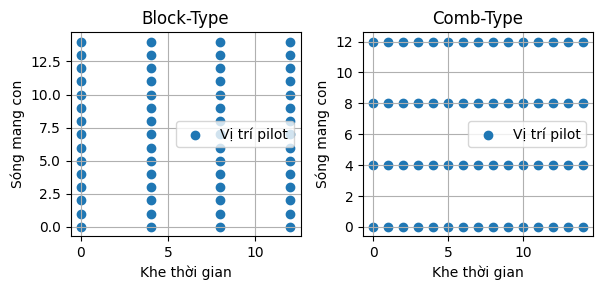
\includegraphics[width=.8\linewidth]{../images/pilot_block_comb.png}
    \caption{Chèn pilot kiểu block-type và comb-type}
\end{figure}

\begin{itemize}
    \item \textbf{Lattice-type}: Pilot được chèn vào theo mô hình hình học (như lưới) trong cả hai miền thời gian và tần số.
\end{itemize}

\begin{figure}[H]
    \centering
    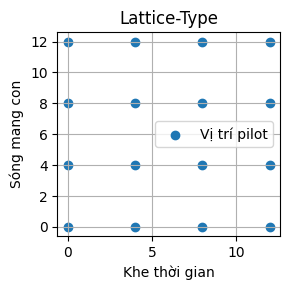
\includegraphics[width=.4\linewidth]{../images/pilot_lattice.png}
    \caption{Chèn pilot kiểu lattice-type}
\end{figure}